\documentclass[10pt,letterpaper]{hitec}
\usepackage{blindtext}
\usepackage[pdftex]{graphicx}
\usepackage{pdfpages}
\usepackage{amsmath}
\usepackage{tikz}
\usepackage{float}
%\usepackage{fullpage}
\usetikzlibrary{shapes, calc, shapes, arrows} 

\author{Keith Herbert}
\title{CMSC 409 - Project 1}
\date{\today}



\begin{document}

\maketitle
\section*{Male and Female Heights}
Figure 1 shows the plot for a set of normally distributed heights generated from mean male and female heights provided by the Wikipedia article on human height\footnote{https://en.wikipedia.org/wiki/Human\_height}
(176.3cm for American males and 163.7cm for American females). The standard deviations for the distributions were taken from a stack overflow topic\footnote{http://biology.stackexchange.com/questions/9730/what-is-the-standard-deviation-of-adult-human-heights-within-sexes} 
as 7cm for males and 6cm for females. The linear separator was estimated to be a horizontal line at 168cm. The equation for this decision function in point-intercept form is $x_1 = 168$, where $x_1$ is the height of an individual in centimeters. This can be rewritten in terms of weights $w_1 x_1 + w_2 = 0$ as $x_1 - 168 = 0$ for $w_1 = 1$ and $w_2 = -168$. 

Table 1 summarizes the results of the classifier. It performs poorly with an error rate of 17.5\% and accuracy just above 82\%. However, it does have a slightly lower false positive rate than the classifier estimated from the height and weight plot (11.7\% vs. 12.4\%)
     

\section*{Male and Female Heights and Weights}
Figure 2 shows the plot for the set of heights generated in the previous section against weights in kilograms calculated by reversing the equation for body mass index (BMI) and normally distributing the BMI according to an article on Pubmed\footnote{http://www.ncbi.nlm.nih.gov/pubmed/23675464} (26.6\% for males and 24.0\% for females, which seems strange --- women should have higher BMI than men. This may be why some of the female weights are freakishly low). Standard deviations for BMI were also taken from the article. All numbers were taken from the 1970s observation wave because students appear to be healthier than the general population. The linear separator was estimated by holding a ribbon up to the screen and observing where it bisected the two groups. The equation calculated from two points on this line was $x_2 = -1.55x_1 + 330$ where $x_1$ is height in centimeters and $x_2$ is weight in kilograms. This can be rewritten in terms of weights $w_1 x_1 + w_2 x_2 + w_3 = 0$ as $1.55x_1 + x_2 - 330 = 0$. for $w_1 = 1.55$, $w_2 = 1$ and $-330$ for the bias $w_3$. 

The results of the classifier are summarized in Table 1. This decision function performs only slightly better than the model trained only with height data. The error is half a percent lower and the accuracy therefor half a percent higher but the true negative for the height and weight classifier is slightly lower for the heigh and weight classifier compared to the height-only separator. The false negative rate does show an improvemnt at being a full percentage point lower, but overall the difference in performance is barely noticable. 

\section*{Conclusion}
Normally distributed height and weight measurements were generated for male and female students with a sample size of two thousand individuals each. Linear classifiers were visually estimated from a plot of just the height data and a plot of both the heights and weights. Results of the classifiers were compared to observe the effect of an extra dimension on the accuracy of a linear classifier. However, the addition of an extra dimension did not make a significant difference in the accuracy and error rates of classification.  

\begin{table*}\centerline{
\begin{tabular}{|l|c|c|}
\hline
               & Height     & Height \& Weight \\
\hline
Error          & 0.17550    &     0.17125   \\
Accuracy       & 0.82450    &     0.82875   \\
True Positive  & 0.44175    &     0.45275   \\
True Negative  & 0.38275    &     0.37600   \\
False Positive & 0.11725    &     0.12400   \\
False Negative & 0.05825    &     0.04725   \\
\hline
\end{tabular}}
\caption{Results for the linear classifiers estimated from the plots of exclusively height measurements and both height and weight measurements. }
\end{table*}


\begin{figure}[p]
\centerline{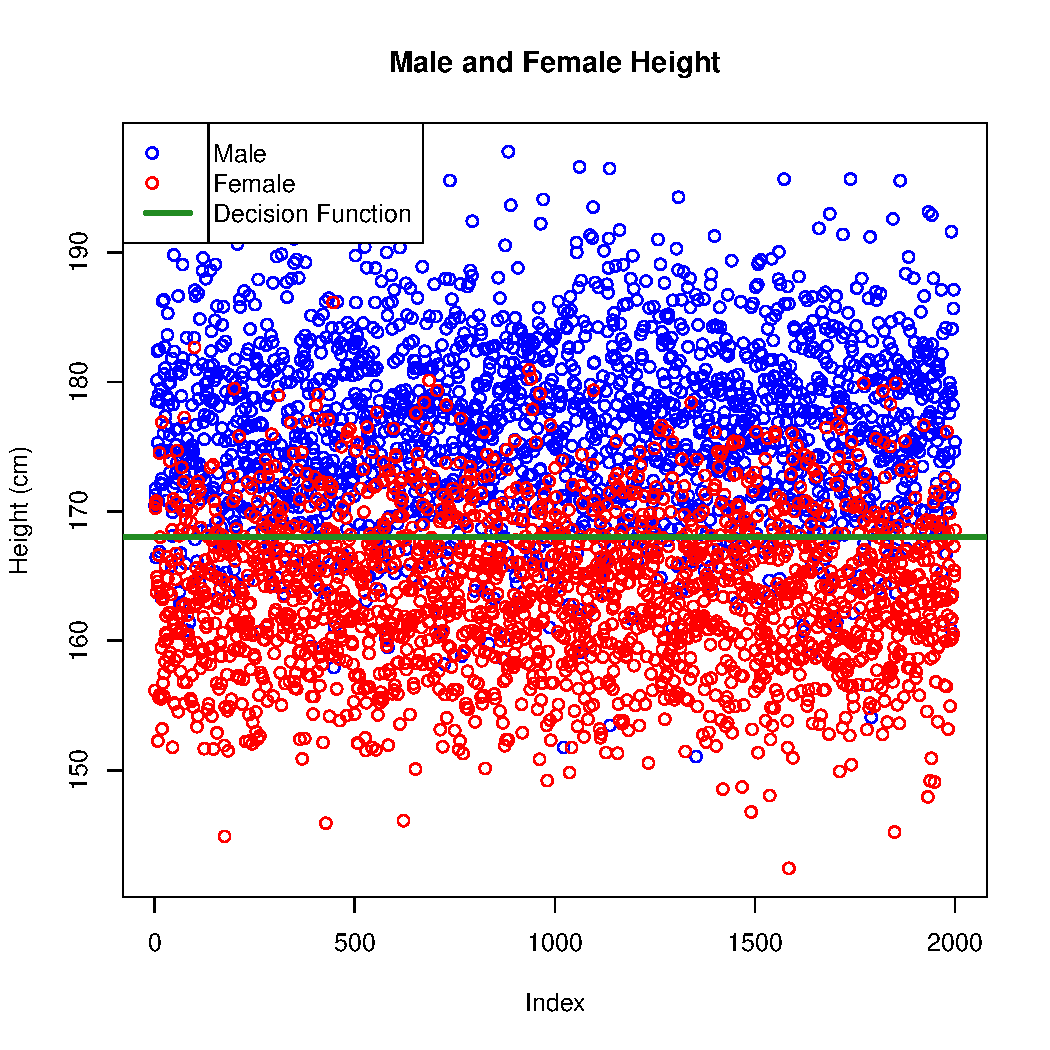
\includegraphics[height=0.9\textheight]{heights.pdf}}
\caption{Scatterplot for the normally distributed heights of 2000 males and 2000 females in centimeters.}
\end{figure}


\begin{figure}[p]
\centerline{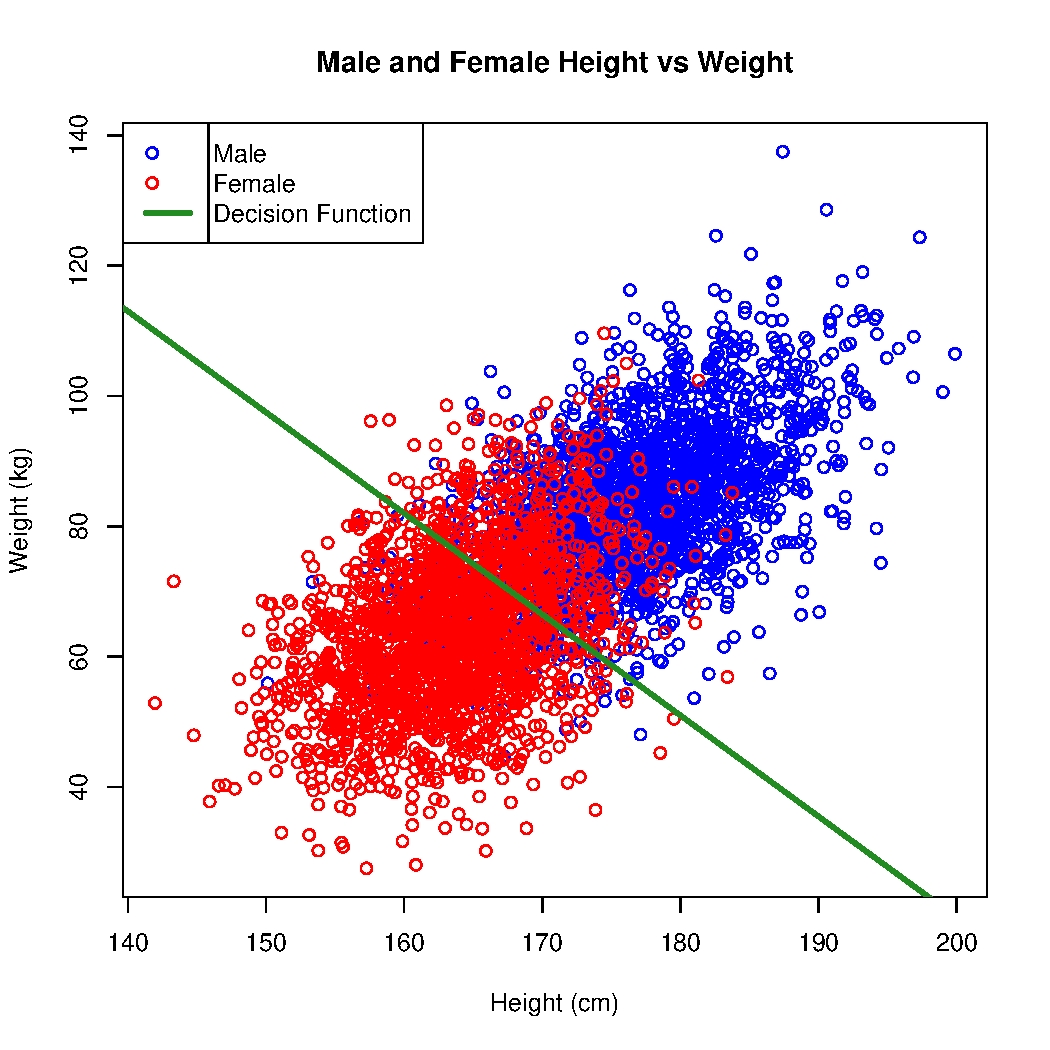
\includegraphics[height=0.9\textheight]{heightsweights.pdf}}
\caption{Scatterplot for the normally distributed heights and weights of 2000 males and 2000 females in centimeters.}
\end{figure}


\end{document}